\documentclass[11pt]{article}


\usepackage[sort]{natbib}
\usepackage{bm,amsmath,bbm,amsfonts,nicefrac,latexsym,amsmath,amsfonts,amsbsy,amscd,amsxtra,amsgen,amsopn,bbm,amsthm,amssymb,graphicx}
\usepackage{wrapfig, caption, subcaption}
\usepackage{fancyhdr}
\usepackage[margin=1.0in]{geometry}
\bibliographystyle{abbrvnat}
\usepackage[section]{placeins}



\title{Fifth Monitoring Committee Meeting \\\vspace{4mm} \normalsize{Understanding the Information Content in Diverse Observations of Forest Carbon Stocks and Fluxes for Data Assimilation and Ecological Modeling\\ NERC CASE partnership with Forest Research}}
\author{\normalsize{E. Pinnington}}
\date{\normalsize{Room ESSC 176, 10am Jan 7, 2016}}


\newtheorem{theorem}{Theorem}[section]
\newtheorem*{defn}{Definition}



	
\begin{document}

\maketitle

\section{Introduction} \label{sec:intro}

Forest ecosystems play an important role in sequestering human emitted carbon-dioxide from the atmosphere and therefore greatly reduce the effect of anthropogenic induced climate change. For that reason understanding their response to climate change is of great importance. Measurements of forest carbon balance are now routinely made in forests across the world using micrometeorological techniques, with many other relevant observations such as leaf area index and standing biomass also available \citep{baldocchi2008turner}. Many efforts have been made to combine this data with models of forest carbon balance using data assimilation techniques in order to improve modelled estimates \citep{zobitz2011primer, fox2009reflex, richardson2010estimating, Quaife2008, Zobitz2014, Niu2014}. Currently, however, the optimal set of observations for understanding the carbon balance of a forest is not known. The aims of this PhD are:

\begin{itemize}
\item Understanding which observations provide models of forest carbon balance with most information in a data assimilation framework, focusing on the CASE partners research site Alice Holt.
\item Finding a better way to quantify background and observation errors and their correlations.
\item Investigating the effect of disturbance on the Alice Holt research forest. The disturbance occured in 2014 when one side of the forest was thinned and the other side left unmanaged. The flux tower measuring net ecosystem exchange of $\text{CO}_{2}$ is situated on the boundary between the two sides. 
\end{itemize}

In the previous report we had decided to move away from work using the Data Assimilation Linked Ecosystem Carbon model (DALEC) and to start using the new version of this model (DALEC2 \citep{Bloom2015}). This was because DALEC2 can be parameterised for both deciduous and evergreen forests, whereas the version of DALEC used in previous work was an evergreen only model. The CASE partners research site (Alice Holt) is a mainly deciduous site. DALEC2 was implemented in a Four-Dimensional Variational data assimilation routine (4D-Var) for joint parameter and state estimation. It was shown that after assimilating 2 years of observations of the Net Ecosystem Exchange (NEE) of CO$_{2}$ from the Alice Holt flux site the forecast (2001-2006) root mean square error between modelled NEE and observed NEE fell from $4.37 \text{gCm}^{-2}\text{day}^{-1}$ to $2.12 \text{gCm}^{-2}\text{day}^{-1}$.

Since completing the previous report, a paper draft has been completed on the work implementing 4D-Var with the DALEC2 model. The final draft of this paper is attached to the monitoring committee report. In this paper the effect that background and observation error statistics and their correlations have on the assimilation have also been investigated. We found that specifying parameter-state error correlations in background error statistics can improve data assimilation forecast results significantly. Including correlations in time between observation error statistics was also found to improve assimilation forecast results. This work was expected to be completed in the new year (2016). However it has been brought forward ahead of completing the observation information content experiments and report.

In the last six months I have also been conducting a field work campaign taking leaf area index measurements at the CASE partners research flux site Alice Holt. These observations will contribute to both the information content experiments and the work investigating the effect of the disturbance on the Alice Holt research forest.       

\section{4D-Var}

In the attached paper draft the DALEC2 functional ecology model is implemented for joint parameter and state estimation. The assimilation routine is then subjected to rigorous testing to check for correctness. We outline novel methods to create a background error covariance matrix (describing our knowledge of the error in prior model estimates before data assimilation) that includes correlations and a novel method to include time correlations between observation errors in the observation error covariance matrix. The background and observation error covariance matrices are largely treated as diagonal in carbon balance model data assimilation. We show that including these correlations can improve forecasts of NEE significantly. The root mean square error in the $14$ year forecast of daily NEE being reduced by $44\%$, decreasing from $4.22~\text{gCm}^{-2}\text{day}^{-1}$ to $2.38~\text{gCm}^{-2}\text{day}^{-1}$. We conducted 4 experiments to investigate the impact of the different matrices on the assimilation. In table~\ref{table:exps_tab} we show which matrices were used in each experiment. 

\begin{table}[ht] 
\begin{center}
	\begin{tabular}{| l | l | l | l | l |}
	\hline
	Experiment & $\textbf{B}_{diag}$ & $\hat{\mathbf{R}}_{diag}$ & $\textbf{B}_{corr}$ &
	$\hat{\mathbf{R}}_{corr}$ \\ \hline
	A & $\times$ & $\times$ & & \\ \hline
	B & & $\times$ & $\times$ & \\ \hline
	C & $\times$ & & & $\times$ \\ \hline
	D & & & $\times$ & $\times$ \\ 
	\hline
	\end{tabular}
	\caption{The combination of error covariance matrices used in each data assimilation experiment. $\textbf{B}_{diag}$ and $\hat{\mathbf{R}}_{diag}$ are the diagonal background and observation error covariance matrices, with no correlations and $\textbf{B}_{corr}$ and $\hat{\mathbf{R}}_{corr}$ are the background and observation error covariance matrices including correlations.}
	\label{table:exps_tab}
\end{center} 
\end{table}

\begin{figure}[ht]
    \centering
    \begin{subfigure}[b]{0.49\textwidth}
        \includegraphics[width=\textwidth]{tdcvt_a.eps}
        \caption{Analysis (Jan 1999 - Dec 1999)}
        \label{fig:td_a}
    \end{subfigure}
    \begin{subfigure}[b]{0.49\textwidth}
        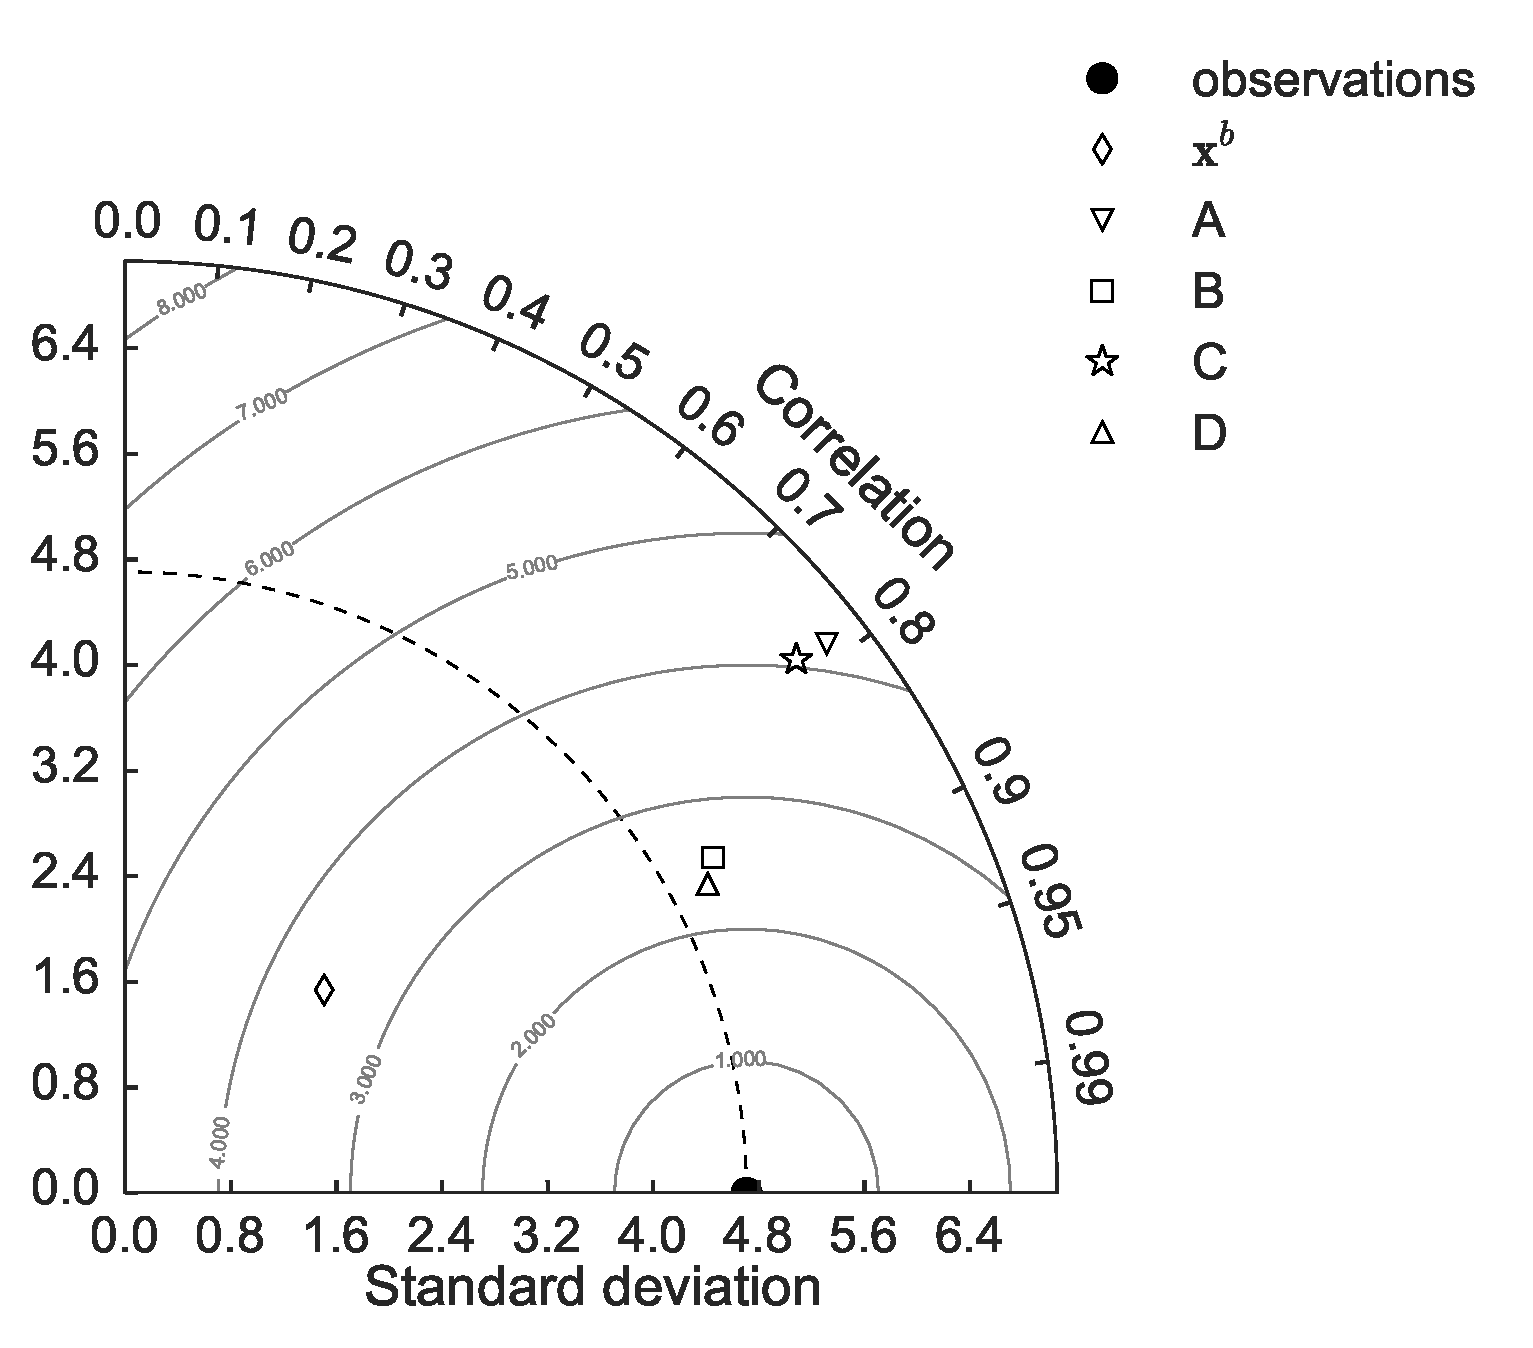
\includegraphics[width=\textwidth]{tdcvt_f.eps}
        \caption{Forecast (Jan 2000 - Dec 2013)}
        \label{fig:td_f}
    \end{subfigure}
    \caption{Taylor diagrams displaying statistical comparison of the four experiment and background analysis (Jan 1999 - Dec 1999) and forecast (Jan 2000 - Dec 2013) results with observations of NEE $( \text{gCm}^{-2}\text{day}^{-1})$. The dotted line represents the standard deviation of the observations and the contours represent values of constant root mean square error between model and observations. Here $\textbf{x}^{b}$ is the background augmented state vector.}
    \label{fig:taylordiag}
\end{figure}

In figure~\ref{fig:taylordiag} we show Taylor diagrams displaying a statistical comparison of the four experiment and background analysis (Jan 1999 - Dec 1999) and forecast (Jan 2000 - Dec 2013) results with the observations of NEE. Here the radial distances from the origin to the points are proportional to the pattern standard deviations and the azimuthal positions give the correlation coefficient between the modelled and observed NEE \citep{Taylor2001}. If a model predicted the observations perfectly it would have a correlation coefficient of $1$ and a radial distance matching that of the observations (represented by the dotted line). Figure~\ref{fig:td_a} shows that all the experiments give very similar results in the analysis window (Jan 1999 - Dec 1999) with all the experiment points closely grouped on top of each other, whereas figure~\ref{fig:td_f} shows the significant difference between the experiment results in the forecast (Jan 2000 - Dec 2013). We see that the model most closely matching the observations is from experiment D where both correlated matrices have been used in the assimilation algorithm.


\section{Field work} \label{sec:fieldwork}

In order to address the third aim of the PhD from section~\ref{sec:intro} a field work campaign has been undertaken to measure Leaf Area Index (LAI) at the Alice Holt flux site. I have used three different methods to measure LAI:
\begin{itemize}
\item Using a ceptometer and an additional Photosynthetically Active Radiation (PAR) sensor. Here we measure below canopy PAR using the ceptometer while logging above canopy PAR using a data logger and PAR sensor positioned outside the canopy. We can then calculate LAI using the above and below canopy readings and a set of equations relying on some assumptions \citep{fassnacht1994comparison}. The ceptometer represents the quickest method for estimating LAI.
\item Using hemispherical photographs as shown in figure~\ref{fig:hemiphotos}. Hemispherical photographs show a complete view of the sky in all directions, from these images we use software which can calculate the proportion of visible sky as a function of sky direction (gap fraction) this can then be used to calculate LAI  \citep{Jonckheere2004}.
\item Using litter traps. Here we place litter traps under the canopy which catch the litter in a bag these bags are changed every week during the litter fall period and the litter sorted into species. We then dry the litter in an oven at $70^{\text{o}}\text{C}$ and weigh it. Towards the end of the season we scan a subsample for each species of 100 leaves  to find an area we then dry and weigh each subsample, a relationship between dry weight and leaf area can then be built and used to infer the total LAI once the whole seasons litter has been collected. This method of LAI calculation is the most time consuming.  
\end{itemize}

For this fieldwork we want to capture both the thinned and unthinned sides of the forest. For this reason I have taken measurements along three transects spanning both sides of the site. Figure~\ref{fig:map} shows a map of the Alice Holt flux site with the three transects and 10m sampling points marked. For the ceptometer I took measurements every 10m giving us 435 readings in total. However the hemispherical photographs were taken every 50m as they are more time consuming. This gave a total of 89 images. I mapped out these points in the forest using a GPS unit and pink tree spray paint. 

I deployed a total of 6 litter traps with 3 positioned in the western side and 3 in the east. However Forest Research already have 10 other traps in operation giving us some valuable extra data. The 6 litter traps is not enough to describe the LAI for the research site \citep{kimmins1973some}. We will use these litter traps as a point of comparison and validation for the ceptometer and hemispherical photograph estimates of LAI made at the same locations. The litter traps have been sampled weekly throughout the autumn and winter which gives us an estimate to the rate of litter fall. This is another observation we can use for data assimilation and model validation.

I have finished taking observations with the ceptometer and hemispherical camera of summer peak LAI. However I am continuing the process of managing the litter traps weekly as this seasons leaf fall period has been longer than usual. I will be taking measurements of spring green up next year in order to constrain the phenology in DALEC2 more accurately. I am now processing the observations I have already taken to find an LAI product. 

At the start of the new year (2016) I will be conducting a biomass survey of the Alice Holt flux site. This will use the method of point centred quarters \citep{dahdouh2006empirical} to determine an estimate of the woody biomass for both sides of the forest. 

We plan to use all observations that I have made and with the available observations of NEE for the thinned and unthinned sides of the forest (partitioned using a flux footprint model) for data assimilation. Two versions of the DALEC2 model will be parameterised (for the thinned and unthinned sides of the forest). This will allow us to see if there is a difference between the optimised parameters for the thinned/unthinned versions of DALEC2. We will test if by just assimilating NEE we can pick out a difference in LAI between the two sides. 

We will investigate the effect of the disturbance further by parameterising DALEC2 for the thinned section of the forest both before and after the thinning occurred using the record of partitioned NEE observations. This will again allow us to see if the optimised parameters are consistent with the known changes to the forest ecosystem.   

\begin{figure}[!ht]
    \centering
    \includegraphics[width=1.\textwidth]{straitsmap_threet_10m.png}
    \caption{Map of the Alice Holt flux site. The crosses are 10m sampling points with the purple diamonds being Forest Research mensuration plots where measurements of woody biomass are made. The black diamond shows the position of the flux tower on the boundary between the thinned (West) and unthinned (East) sides of the forest.}
    \label{fig:map}
\end{figure}


\begin{figure}[!h]
\centering
\begin{subfigure}{.5\textwidth}
  \centering
  \includegraphics[width=.7\linewidth]{043exp2.jpg}
  \caption{Unthinned}
  \label{fig:sub1}
\end{subfigure}%
\begin{subfigure}{.5\textwidth}
  \centering
  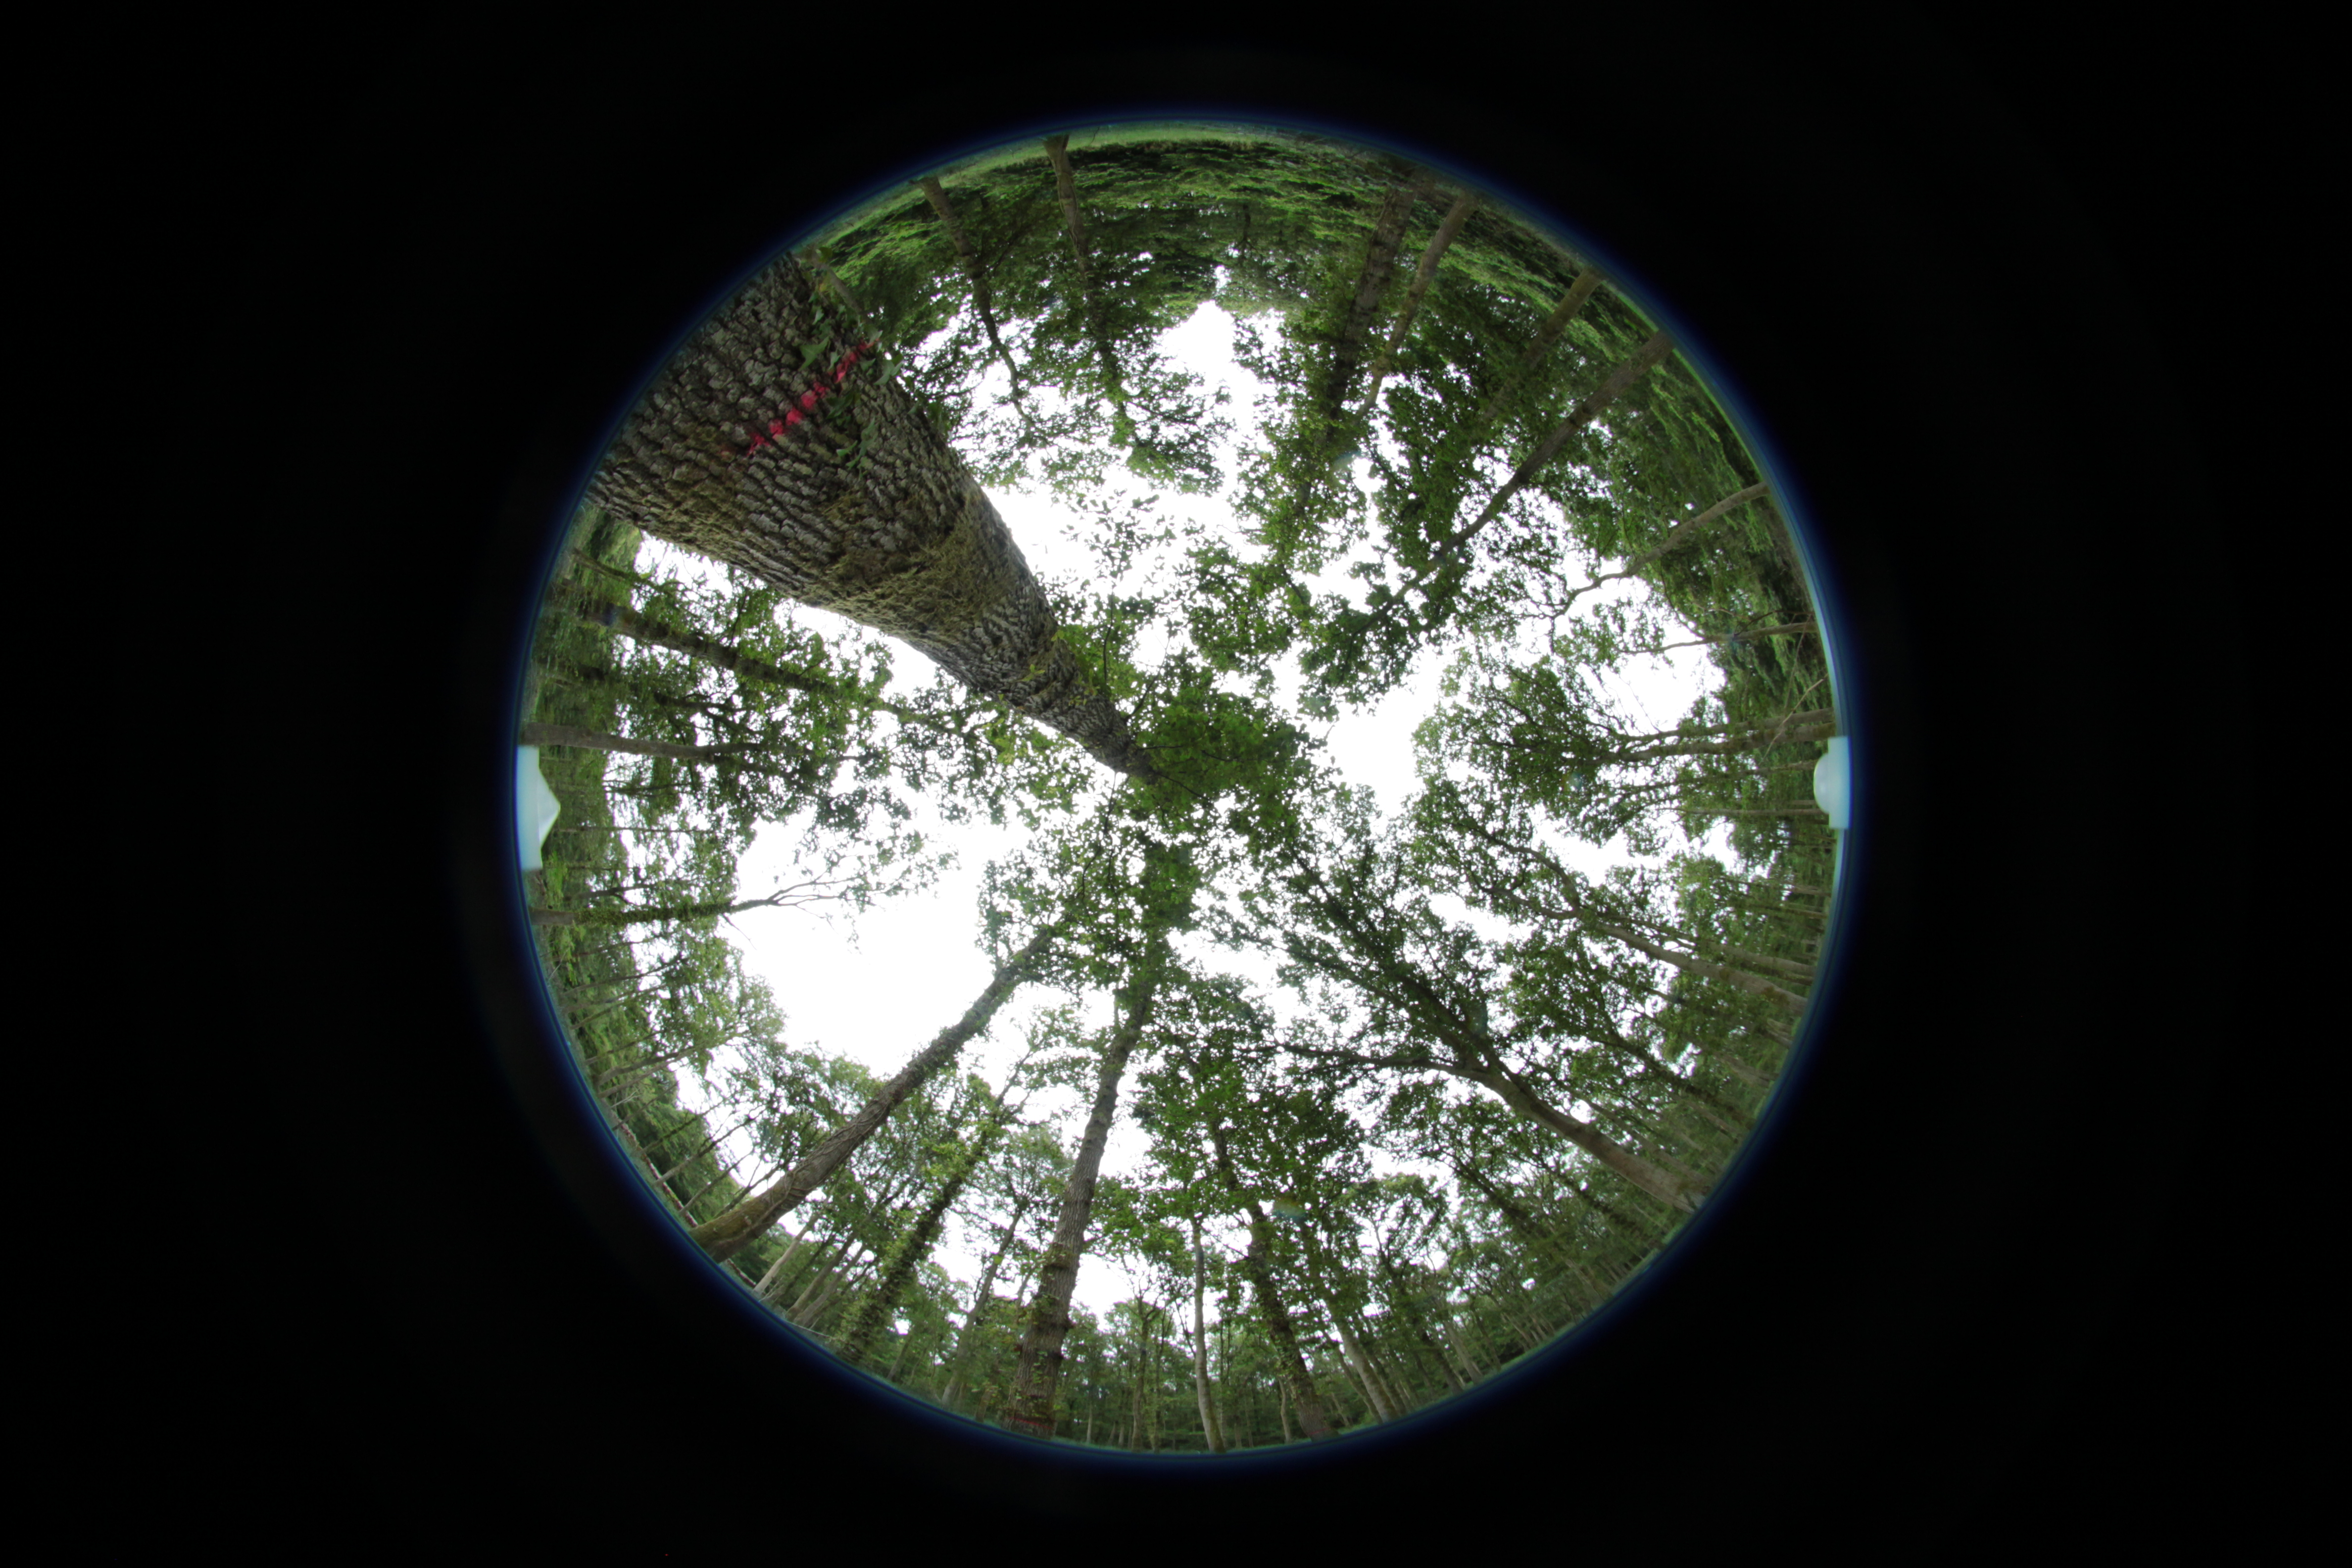
\includegraphics[width=.7\linewidth]{252exp1.jpg}
  \caption{Thinned}
  \label{fig:sub2}
\end{subfigure}
\caption{Hemispherical photographs from the Alice Holt flux site showing the difference between the thinned and unthinned sides of the forest.}
\label{fig:hemiphotos}
\end{figure}

\section{Current work and future plans}

I am currently in the process of getting the attached paper finished and we hope to have it submitted early in the new year (2016). I have begun repeating the information content experiments using DALEC2. these experiments had been previously conducted using the original DALEC model. In addition to the measures previously used for DALEC (SIC and DFS), I will be extending this work to include other measures. The influence matrix measures the sensitivity of the analysis in observation space to the observations \citep{Cardinali2004}. The adjoint technique proposed by \cite{Langland2004}, approximates the sensitivity of a scalar forecast error norm to the observations . In \cite{Cardinali2004} the data assimilation problem is assumed to be Gaussian with a linear function mapping the state to observation space (\textbf{H}), such that,
\begin{equation}
\textbf{x}_{a} = \textbf{x}_{b} + \textbf{K}(\textbf{y} - \textbf{H}\textbf{x}_{b}), \label{daupdate}
\end{equation}
where \textbf{K} is the Kalman gain matrix, $\textbf{K} = (\textbf{H}^{T}\textbf{R}^{-1}\textbf{H} + \textbf{B}^{-1})^{-1}\textbf{H}^{T}\textbf{R}^{-1}$. The influence matrix is then defined as,
\begin{equation}
\textbf{S} = \frac{\partial {\mathbf{H}}\textbf{x}_a}{\partial {\textbf{y}}} = \textbf{K}^{T}\textbf{H}^{T}. \label{influmat}
\end{equation}
In order to consider observations over a 4D-Var time window we rewrite equation~\ref{daupdate} as,
\begin{equation}
\textbf{x}_{a} = \textbf{x}_{b} + \hat{\textbf{K}}(\hat{\textbf{y}} - \hat{\textbf{H}}\textbf{x}_{b}), \label{ass_xa}
\end{equation}
using the defined matrices in the attached paper, with $\hat{\textbf{K}} = (\hat{\textbf{H}}^{T}\hat{\textbf{R}}^{-1}\hat{\textbf{H}} + \textbf{B}^{-1})^{-1}\hat{\textbf{H}}^{T}\hat{\textbf{R}}^{-1}$. Equation~\ref{influmat} then becomes,
\begin{equation}
\textbf{S} = \frac{\partial {\hat{\mathbf{H}}}\textbf{x}_a}{\partial \hat{{\textbf{y}}}} = \hat{\textbf{K}}^{T}\hat{\textbf{H}}^{T}. \label{influmat2}
\end{equation}
In equation~\ref{ass_xa} we have also assumed that we have a linear model, $\mathbf{M}_{i,0}$, evolving our state from time 0 to time $i$. We know that our model is in fact nonlinear but have tested the tangent linear hypothesis for DALECV2 in the attached paper and have seen it to be a good approximation. 

Using these measures and an observing system simulation experiment that I have developed, I will produce another report investigating the best set of observations for understanding the carbon balance of a forest. We will explore the impact of using the correlated background and observational error covariance matrices defined in the attached paper on these information content measures. Using the twin experiments we will also investigate the effect of the correlated error covariance matrices on recovering the truth after assimilating a set of synthetic observations. I am also continuing with the fieldwork campaign as described in section~\ref{sec:fieldwork}. I have currently processed the ceptometer data to produce a Fraction of Absorbed Photosynthetically Active Radiation (FAPAR) product as shown in figure~\ref{fig:fapar}. Work to produce an LAI product is still ongoing. From figure~\ref{fig:fapar} we can see that the FAPAR produce demonstrates the distinct difference in canopy structure for the different sections of the forest site. Other future work will be based on the attached thesis outline and Gantt chart. 


\begin{figure}[!ht]
    \centering
    \includegraphics[width=.8\textwidth]{ahfapar2.pdf}
    \caption{Map of the Alice Holt flux site displaying values of FAPAR for the 10m sampling points of the ceptometer in the described field work campaign in section~\ref{sec:fieldwork}.}
    \label{fig:fapar}
\end{figure}


\section{Professional and Academic Development}

\subsection{Masters Courses}
\begin{itemize}
\item MAMB10 (Data Assimilation) - 85\%
\item MAMNSO (Numerical Solutions to Ordinary Differential Equations) - 79\%
\item MTMG02 (Atmospheric Physics) - 66\%
\item MTMG49 (Boundary Layer) - 72\%
\item MTMD01 (Environmental Data Visualization) - 78\%
\item MTMD02 (Operational Data Assimilation) - 70\%
\end{itemize}

\subsection{Transferable Skills}

During my PhD I have taken part in the following courses, workshops and activities:
\begin{itemize}
\item 28/01/2014 - Basic Statistics Refresher - RRDP

\item 31/03/2014-01/04/2014 - Land Data Assimilation workshop at UCL - ESA

\item 23/04/2014-25/03/2014 - Correlated Observation Errors in Data Assimilation Workshop - ESA

\item 13/05/2014 - Social Media - Bloggs, Twitter and Your Online Presence - RRDP

\item 29/05/2014 - How to Write a Paper - RRDP

\item 25/06/2014-26/06/2014 - Software Carpentry Course - Git and Python

\item 10/07/2014-11/07/2014 - Forest Research - Helped with field work LiDAR

\item  21/07/2014-01/08/2014 - Fluxcourse Summer School - University of Colorado

\item 29/09/2014-03/10/2014 - NERC course - Software Development for Environmental Scientists Level 1

\item 08/10/2014-10/10/2014 - Environment YES - NERC ``dragon's den" type competition at Syngenta, Jesops Hill

\item 17/12/2014 - Presentation at Maths for Planet Earth Industry day

\item 24/02/2015 - Reading Soil Centre Workshop - What can Land Surface Models do for you?

\item 23/03/2015-27-03/2015 - NERC course - Software Development for Environmental Scientists Level 2

\item 11/03/2015 - Quo Vadis presentation

\item 08/09/2015-11/09/2015 - RSPSoc conference University of Southampton - Presented a poster

\item 24/09/2015 - Department poster presentation - Recieved an honourable mention for poster on ``Understanding the information content in observations of forest carbon balance"

\item 02/11/2015-03/11/2015 - BES Ecosystems and Climate Change Mitigation Conference, Charles Darwin House, London - Presented a poster

\item 02/12/2015 - RMetS SE centre meeting, Reading Town Hall - Invited to give a presentation after receiving honourable mention at the department poster presentation
\end{itemize}

\subsection{Demonstrating}
During my PhD I have helped demonstrate on the following courses:
\begin{itemize}
\item 15/09/2014-1909/2014 - NERC Data assimilation for environmental scientists training course

\item 16/02/2015-20/02/2015 - NERC Software Development for Environmental Scientists Level 1

\item 20/04/2015-23/04/2015 - MT26E Surface Energy Exchange Practicals
\end{itemize}


\bibliography{../../PhD}{}
%\bibliographystyle{plain}
\end{document}